% Este arquivo .tex será incluído no arquivo .tex principal. Não é preciso
% declarar nenhum cabeçalho

\section{CACo -- Centro Acadêmico da Computação}

\begin{figure}[H]
    \centering
    
\includegraphics[width=.35\textwidth]{img/caco_logo.pdf}
\end{figure}

Bix*, o CACo é o seu centro acadêmico. Um CA é uma entidade estudantil que, em
linhas gerais, deve trabalhar para garantir os interesses d*s estudantes e
melhorar o curso e a faculdade a que pertence. O CACo é formado pel*s alun*s de
graduação tanto em Engenharia quanto em Ciência da Computação da Unicamp, bem
como *s alun*s de pós-graduação do IC. Tod* e qualquer alun* desses cursos é
membro do CACo e isso inclui você.

Um centro acadêmico é parte do famoso ''movimento estudantil'' de que você
provavelmente já ouviu falar. Mas não se engane! Pergunte para o seu pai o que
ele pensa quando lê ''movimento estudantil'' e ele vai dizer que vê um bando de
estudantes desocupad*s associad*s a um partido político de esquerda que saem por
aí protestando contra o sistema e queimando ônibus pelas ruas. Se você pensa
assim, mude sua ideia: o CACo não é nada disso.

\begin{figure}[H]
    \centering
    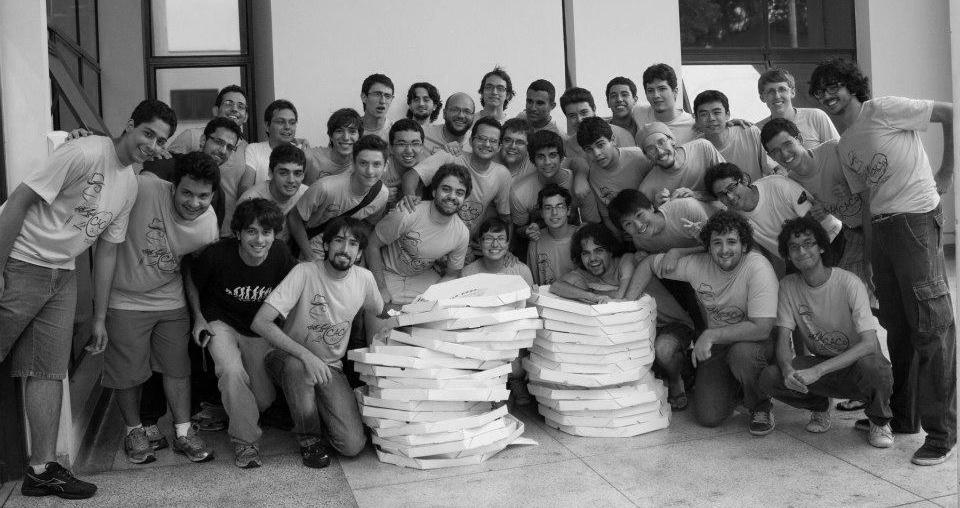
\includegraphics[width=.45\textwidth]{img/alem_da_graduacao/caco_pizzada1.jpg}
\end{figure}

O CACo tem como função representar *s estudantes no âmbito acadêmico, ou seja,
perante o IC, a FEEC e a Unicamp. Mas o que o CACo faz? De forma simplificada,
procuramos ser porta-voz d*s alun*s. Reivindicamos espaço físico decente para *s
alun*s, alteração nas matérias e professor*s, promovemos discussões sobre temas
polêmicos e delicados, dentre muitas outras atividades.

Quer um exemplo? Esse estupendo manual que você está lendo neste exato momento
foi confeccionado pelo seu centro acadêmico para lhe ajudar no início da sua
vida universitária e, na verdade, você ainda vai se pegar recorrendo ao seu
manual várias vezes durante seus quatro, cinco, doze anos na Unicamp.

Uma grande função do CACo é prezar pela qualidade dos cursos e fazemos isso, por
exemplo, através de discussões com o próprio Instituto, onde levamos reclamações
e reivindicações d*s alun*s para*s coordenador*s e professor*s.

\begin{figure}[H]
    \centering
    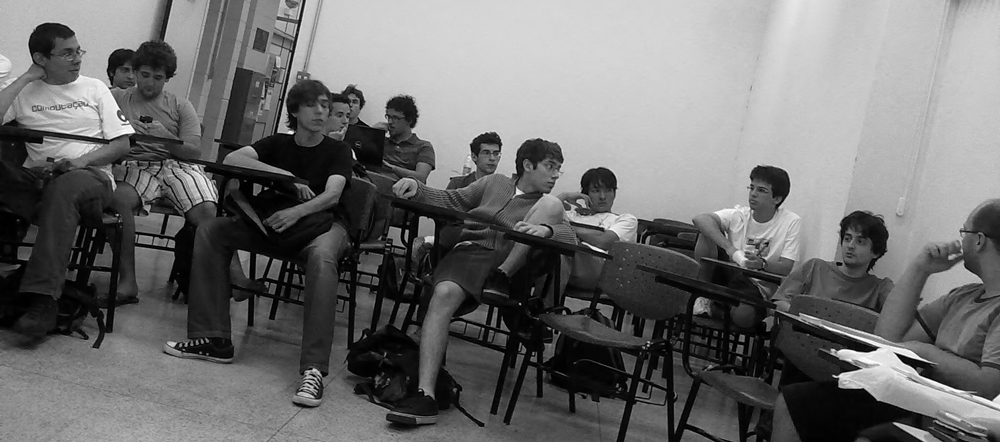
\includegraphics[width=.45\textwidth]{img/alem_da_graduacao/caco_reuniao.jpg}
\end{figure}

Uma outra função do CACo é integrar *s estudantes de computação da Unicamp. Para
isso, realizamos diversos eventos como o CineCACo, o PipoCACo, o CACo Games, o
CACo Series of Poker e a grande comemoração do Aniversário do CACo, que contou
com pizza de graça para mais de duzentos alun*s! Tentamos também facilitar a
vida da galera através dos armários que alugamos, o Banco de Livros e o Banco de
Provas, o maior da Unicamp, disponível online.

Repetindo o que foi dito antes: bix*, o CACo é o \textbf{seu} Centro Acadêmico.
Tudo que dissemos que fazemos pel*s alun*s, queremos fazer por você também. Por
isso, quando houver algum problema envolvendo a FEEC, o IC, *s professor*s ou
qualquer coisa do tipo, não hesite em nos procurar. O CACo sempre lhe dará todo
o suporte necessário. Se tiver reclamação ou sugestão relacionada ao próprio
CACo, também estaremos aqui para ouvir. Mais do que isso, venha participar de
uma de nossas reuniões, que são abertas a você e tod*s *s alun*s de computação
da Unicamp.

\begin{figure}[H]
    \centering
    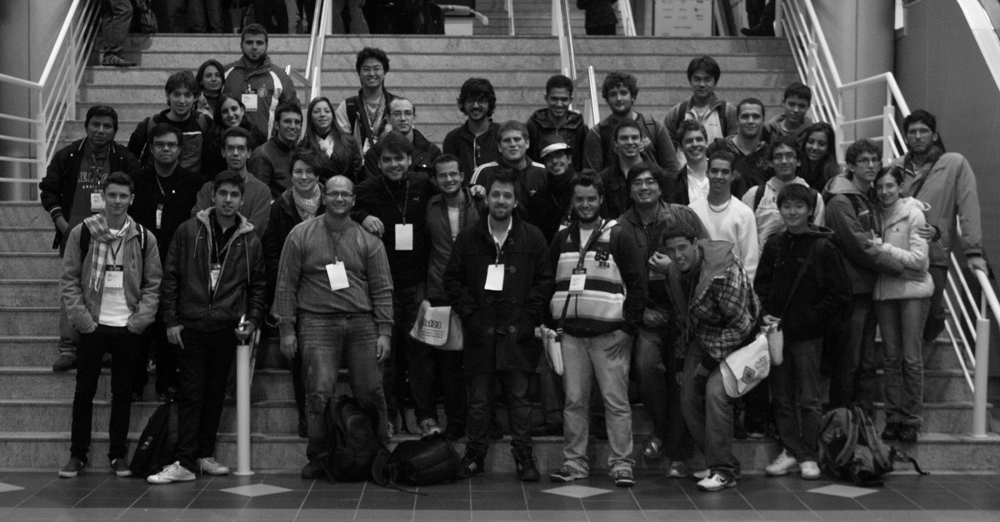
\includegraphics[width=.45\textwidth]{img/alem_da_graduacao/caco_fisl2.jpg}
\end{figure}

Participar do CACo é uma experiência diferente de tudo aquilo que você terá na
sua graduação. É a chance de aprender e crescer de uma forma que não acontece em
nenhuma aula de cálculo. É uma oportunidade de conhecer seus(suas) veteran*s e também
seus(suas) amiguinh*s bix*s. Mas, acima de tudo, é uma experiência pessoal onde você
vai aprender a se expressar, argumentar, defender suas ideias, falar em público
e pensar no coletivo. Você entrará em contato com muita gente que provavelmente
você nunca iria conhecer e, com certeza, fará amizade com muit*s del*s. Por
esses e muitos outros motivos é que você, bix*, deve vir a pelo menos uma
reunião do CACo e sentir na pele tudo o que foi dito aqui. Venha nos ajudar a
fortalecer ainda mais o melhor CA da Unicamp. Até a reunião!

\begin{compactitemize}
    \item  E-mail: \email{caco@ic.unicamp.br}
    \item  Site: \url{www.caco.ic.unicamp.br}
    \item  Reuniões: você será informad* no começo do semestre sobre os horários
        das reuniões. Participe!
\end{compactitemize}

Veja a seguir algumas das atividades que o CACo pratica:

\subsection{Avaliação de Curso e Reforma Curricular}

Uma vez por semestre, ocorre a reunião de avaliação de curso da qual participam
alun*s, coordenador*s e professor*s, além de responsáveis pela infraestrutura do
IC e da FEEC. Nela, são discutidos problemas relativos aos cursos, que vão desde
professor*s ruins até cadeiras quebradas. São avaliadas as disciplinas,
apontados problemas e indicadas soluções. A participação dos alun*s é muito
importante, afinal somos nós que mais ganhamos e perdemos com o bom e o ruim de
nossos cursos. Por isso, o CACo participa dessa reunião levando a opinião d*s
alun*s para serem debatidas.

A avaliação de curso também visa a reforma curricular dos cursos. O catálogo do
curso (disciplinas que devem ser cursadas) é alterado todos os anos e a reunião
de avaliação tem grande papel nessas alterações.

\subsection{Caravana para o FISL}

O CACo organiza anualmente uma caravana para o FISL, o Fórum Internacional de
Software Livre, que acontece em Porto Alegre. O FISL reúne milhares de pessoas
de todo o mundo e conta com palestras e profissionais de renome. O Fórum é um
ótimo modo de entrar em contato com o mundo da computação e a caravana é uma
ótima e barata maneira de ir e tembém de socializar com outr*s computeir*s.

\begin{figure}[H]
    \centering
    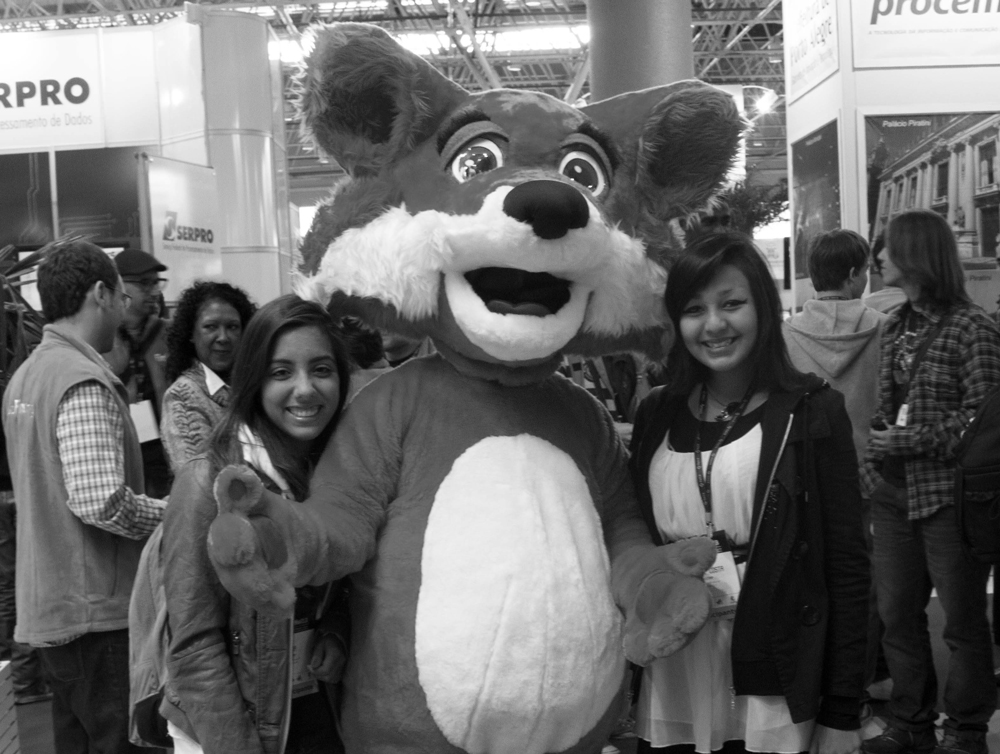
\includegraphics[width=.45\textwidth]{img/alem_da_graduacao/caco_fisl1.jpg}
\end{figure}

\subsection{Pesquisa Salarial}

Em 2010, com a colaboração do diretor do IC, o professor Hans Liesenberg, e da
rede social Reunion, promovemos uma pesquisa salarial com ex-alun*s de
computação, que ajudou a fornecer um bom panorama da realidade em que se
encontra o profissional formado pela Unicamp na área de computação. A pesquisa
está disponível no site do CACo.

\subsection{CineCACo}

Por que não juntar com a galera no IC para assistir um filme com pipoca e
refriegerante de graça?

\subsection{PipoCACo}

Os PipoCACos são eventos de discussão sobre assuntos polêmicos, mas sem
comentários sobre  mamilos. Trata-se de um espaço para que toda a Computação
possa discutir um assunto de interesse geral. Por exemplo, já realizamos
PipoCACos sobre cotas em universidades públicas, sobre o Enade e semestralmente
fazemos o PipoCACo de Avaliação de Curso, onde reunimos as reclamações d*s
alun*s para a reunião de avaliação. Além de um ótimo local para ouvir opiniões e
debater, os PipoCACos são regados a refrigerante e pipoca por nossa conta!

\subsection{LariCACo}

Bateu aquela fome e não tem lugar perto pra comer? Vá até o LariCACo!
Devido ao IC ficar muito distante das lanchonetes presentes na Unicamp, em 2015
criamos o LariCACo, que é basicamente a venda de comida dentro do IC. Ele
funciona em um esquema de auto-atendimento, onde você escolhe em uma tabela de
produtos e preços o que quer comer e deposita o dinheiro dentro da nossa caixa
gabinete, simples assim! O LariCACo fica dentro da salinha do CACo, no IC, 
e sempre é reabastecido pelos membros do CACo. 

\subsection{Palestra AA/AB}

Chega um momento na vida de tod* computeir* engenheir* em que el* deve responder
às questões fundamentais como: De onde viemos? Para onde vamos? Onde vamos
almoçar hoje? Vou ser Azóide ou Bzóide?

O curso de Engenharia de Computação da Unicamp se divide em duas habilitações,
também conhecidas como modalidades: AA e AB. A diferença? Não é simples! Por
isso, o CACo organiza uma série de palestras a fim de ajudá-l* a escolher a
modalidade que mais lhe agrada.

\subsection{CACo Series of Poker}

O lendário torneio de Poker do CACo. Aberto a toda a computação, o CSoP é um
ótimo evento de integração e já contou com oito edições de absoluto sucesso!
Você será informad* da data do próximo, fique ligad*!

\begin{figure}[H]
    \centering
    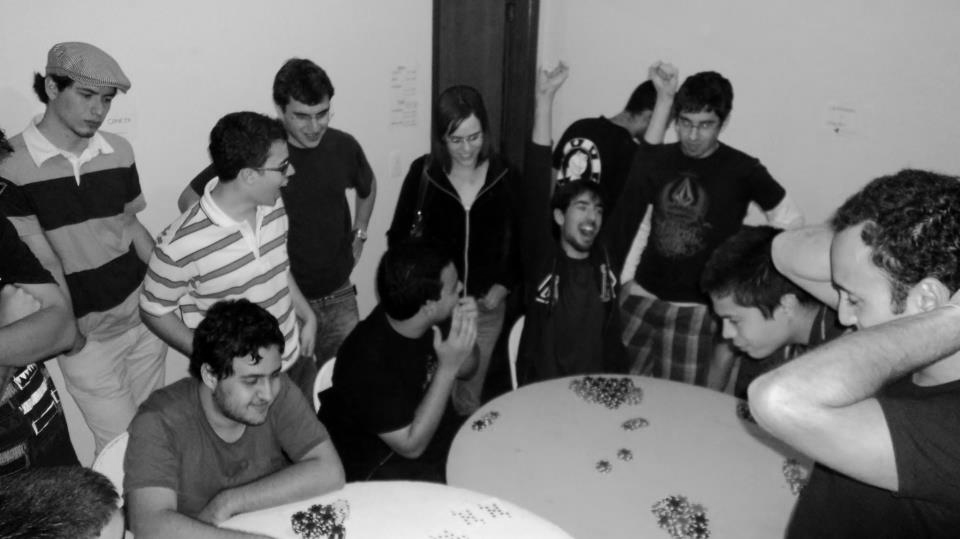
\includegraphics[width=.45\textwidth]{img/alem_da_graduacao/caco_poker2.jpg}
\end{figure}

\subsection{Salinha}

A sede do CACo fica na nossa salinha no IC-3. Munida de uma incrível mesa de
sinuca, ela está aberta 24/7 para tod*s *s computeir*s que queiram jogar.

\subsection{Atendimento}

O CACo realiza atendimentos na nossa salinha. Nesses horários, você poderá
comprar nossos produtos, se inscrever em algum de nossos eventos ou só bater
papo com a gente mesmo. Os horários de atendimento serão divulgados no início do
semestre e você pode conferi-los no site do CACo.

\begin{figure}[H]
    \centering
    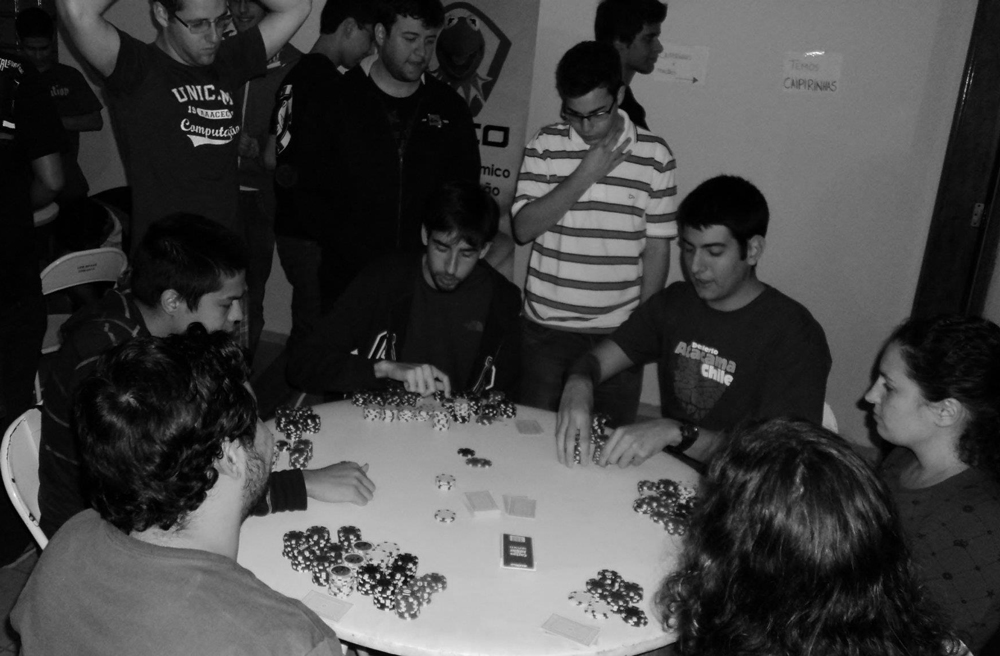
\includegraphics[width=.45\textwidth]{img/alem_da_graduacao/caco_poker1.jpg}
\end{figure}

\subsection{Manual do Bixo}

Esse excelente manual que você está lendo agora não caiu do céu. Em tempos
imemoriais, o Manual do Bixo era feito pela Atlética, porém atualmente o CACo
assumiu a responsabilidade de editar, imprimir e distribuir o Manual aos
ingressantes todos os anos. Utilizamos Git pra controle de versão e {\LaTeX }
para formatação do conteúdo. Para contribuir, o melhor jeito é mandar pull
requests para nosso repositório, \url{github.com/cacounicamp/Manual-do-Bixo},
mas você também pode mandar um email pra gente com as contribuições caso você
não saiba usar Git ou \LaTeX.

\subsection{Gestão}

O CACo tem uma gestão composta de gente bonita e charmosa. Não se preocupe, se
você não é bonit* nem charmos*, você ainda pode entrar na gestão... talvez. A
atual gestão foi eleita em novembro de 2015 e deve permanecer até outubro de
2016. Mas não pense que só a gestão gere o CACo. Mais uma vez: o CACo é o seu
centro acadêmico. Você e toda a computação também fazem parte do CACo e têm
papel nas nossas decisões e discussões.

Para ficar mais integrado ao que ocorre no seu centro acadêmico, como suas
ações, projetos e quais os problemas atuais, você pode se increver na lista do
CACo no Google Groups por meio do link:
\url{bit.ly/cacounicamp}.

\begin{figure}[H]
    \centering
    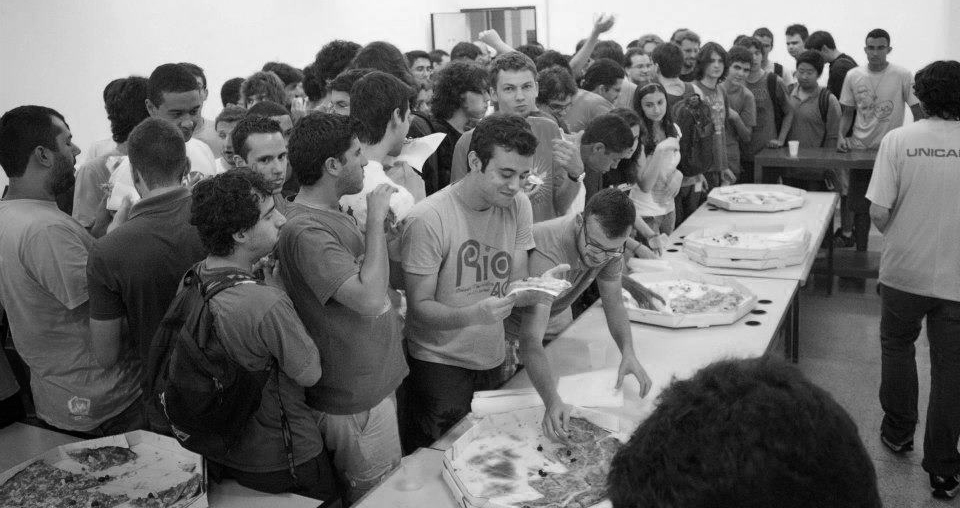
\includegraphics[width=.45\textwidth]{img/alem_da_graduacao/caco_pizzada2.jpg}
\end{figure}

\begin{figure}[H]
    \centering
    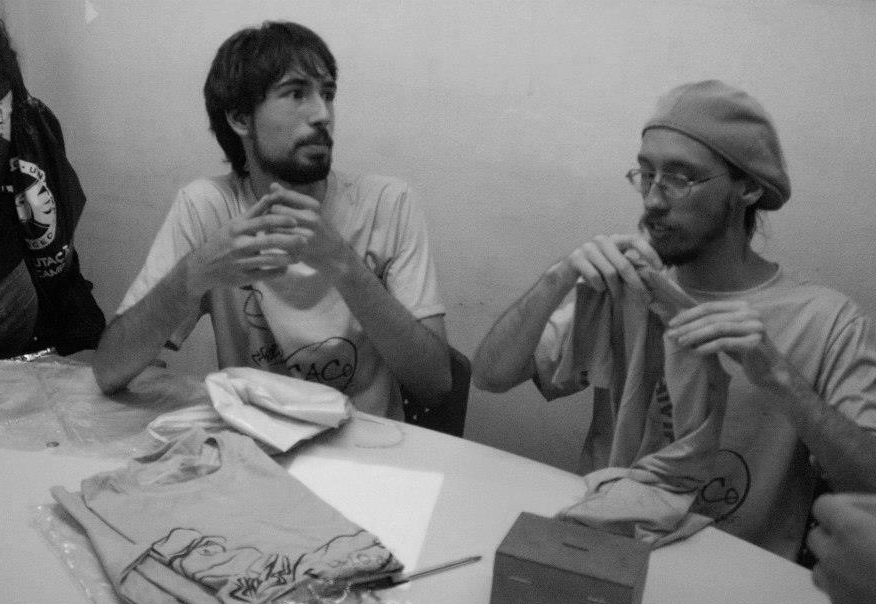
\includegraphics[width=.45\textwidth]{img/alem_da_graduacao/caco_eleicao.jpg}
\end{figure}

\subsubsection*{Chapa ''Capichapa'' (2015/2016)}

\begin{itemize}
    \item   \textbf{Presidência}
        \\Lucas Silva Schanner (Capiva EC014)

    \item   \textbf{Coordenadoria Administrativa}
        \\Guilherme Lucas da Silva (Virose EC014)
        \\Ana Carolina Requena Barbosa (EC015)
        \\Henrique Noronha Facioli (EC014)
        \\Daniel Helú Prestes de Oliveira (EC015)

    \item   \textbf{Coodenadoria Financeira}
        \\Lauro Cruz e Souza (Peta EC014)
        \\Ignácio Espinoso Ribeiro (Lula EC015)

    \item   \textbf{Coordenadoria de Ensino e Graduação}
        \\Yuri Corrêa Pinto Soares (CC012)
        \\João Victor Brazileu Spuri (Logan EC015)
        
    \item   \textbf{Coordenadoria de Eventos}
        \\André Figueiredo de Almeida (Monopoly CC015)
        \\Gustavo Fernandez da Costa (Frodo EC015)
        \\Andreza Aparecida dos Santos (EC015)

    \item   \textbf{Coordenadoria de Produtos, Comunicação e Marketing}
        \\Alex Wei (EC014)
        \\Eduardo Moreira Freitas de Souza (Chamyto EC015)

    \item    \textbf{Coordenadoria Tecnológica}
        \\Lucas de Camargo Barros de Castro (Foo EC015)
        \\Eric Ribeiro Daher (EC015)
        \\Giovani Nascimento Pereira (Viagra EC015)
\end{itemize}

As gestões dos anos anteriores podem ser vistas no site do CACo.

\begin{figure}[H]
    \centering
    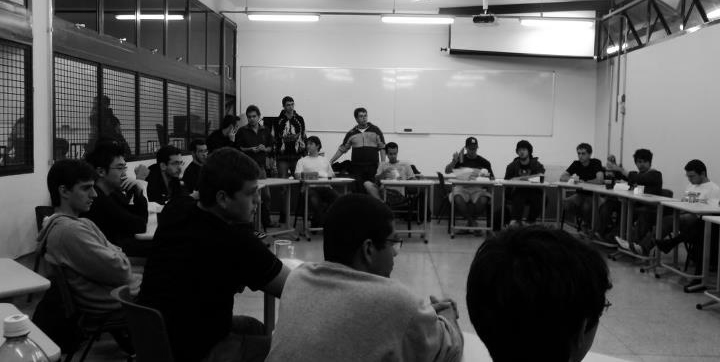
\includegraphics[width=.45\textwidth]{img/alem_da_graduacao/caco_pipocaco.jpg}
\end{figure}
